\chapter{Approach}\label{chapter:Approach}
\section{Requirement Analysis and Technology Comparison}

\subsection{Requirement Analysis}

To determine the most suitable solution, a comprehensive requirement analysis is essential. This analysis will also serve to evaluate the effectiveness of the chosen approach and identify any trade-offs made during implementation.

\subsubsection{Library Complexity}

The sys\_sage library, as outlined in the terminology section, exhibits significant complexity, encompassing a multitude of functions. Many of these functions are designed to modify object states and retrieve information about components or the overall topology. The mapping of basic C++ data types to their Python counterparts should be straightforward. Components and Datapaths feature attribute maps, enabling the addition of custom attributes. It is crucial that these attribute maps are accessible from Python, allowing users to define and manipulate custom attributes.

The library also manages horizontal and vertical connections through component parent-child relationships and datapath source-target relationships. The Python implementation must handle all objects with precision, mirroring the execution behavior of the C++ functions. Sys\_sage employs inheritance, with classes like Topology inheriting from the generic Component class. While Python supports inheritance, the integration of inheritance and polymorphism requires careful consideration to avoid potential workarounds. This aspect will be addressed in this work, particularly concerning the generalization of the Datapaths class to accommodate future specific Datapaths types.

Sys\_sage supports up to three external interfaces: intel\_pqos, nvidia\_mig, and proc\_cpuinfo. The Python bindings should allow users to utilize these interfaces when available and desired. Additionally, sys\_sage provides XML import and export functionality, enabling users to customize attribute import and export processes.

\subsubsection{Performance}

The most computationally intensive tasks involve searching and updating components within the topology. The time required for these operations increases with the size of the component. To minimize overhead, the Python bindings should primarily rely on the existing C++ functions, avoiding reimplementation in Python.

\subsubsection{Library Dependency}

The chosen approach should minimize external dependencies to streamline the installation process and enhance user experience. Excessive dependencies can lead to installation complexities, conflicts, and maintenance challenges.

\subsubsection{Error Handling and Documentation}

While performance considerations might lead to reduced emphasis on error handling, comprehensive documentation is vital. The documentation should clearly delineate the capabilities and limitations of the Python bindings.

\subsubsection{Future Support}

Long-term support and maintainability are crucial. The implementation should be easily understandable and modifiable, even by developers unfamiliar with the project.

\subsubsection{Build and Installation}

Users should have the option to install the library with or without Python accessibility.

\subsubsection{User Experience}

Python programmers, who may not be accustomed to the intricacies of C++ programming, require an interface that is intuitive and robust. The bindings must prevent errors arising from misuse, such as segmentation faults, by providing clear error messages and idiot-proof functions.

\subsection{Technology Evaluation for Python Integration}

Several technologies were considered for their potential to facilitate the integration of our C++ library with Python. Each option presents a unique set of features and trade-offs concerning performance, ease of implementation, and compatibility with modern C++ constructs.
Furthermore we provided some sketches that show which steps are involved to use the technologies in a project. These illustrations should only give a rough idea behind the application of the different options.

\subsubsection{ctypes: Direct Library Interaction}

ctypes enables Python to directly interface with dynamic link libraries, providing access to C-compatible data types and functions. While straightforward for basic C interactions, it necessitates manual type conversions and lacks native support for C++ object-oriented features. This can complicate the wrapping of libraries with complex C++ structures and inheritance.

\begin{figure}[htpb]
    \centering
    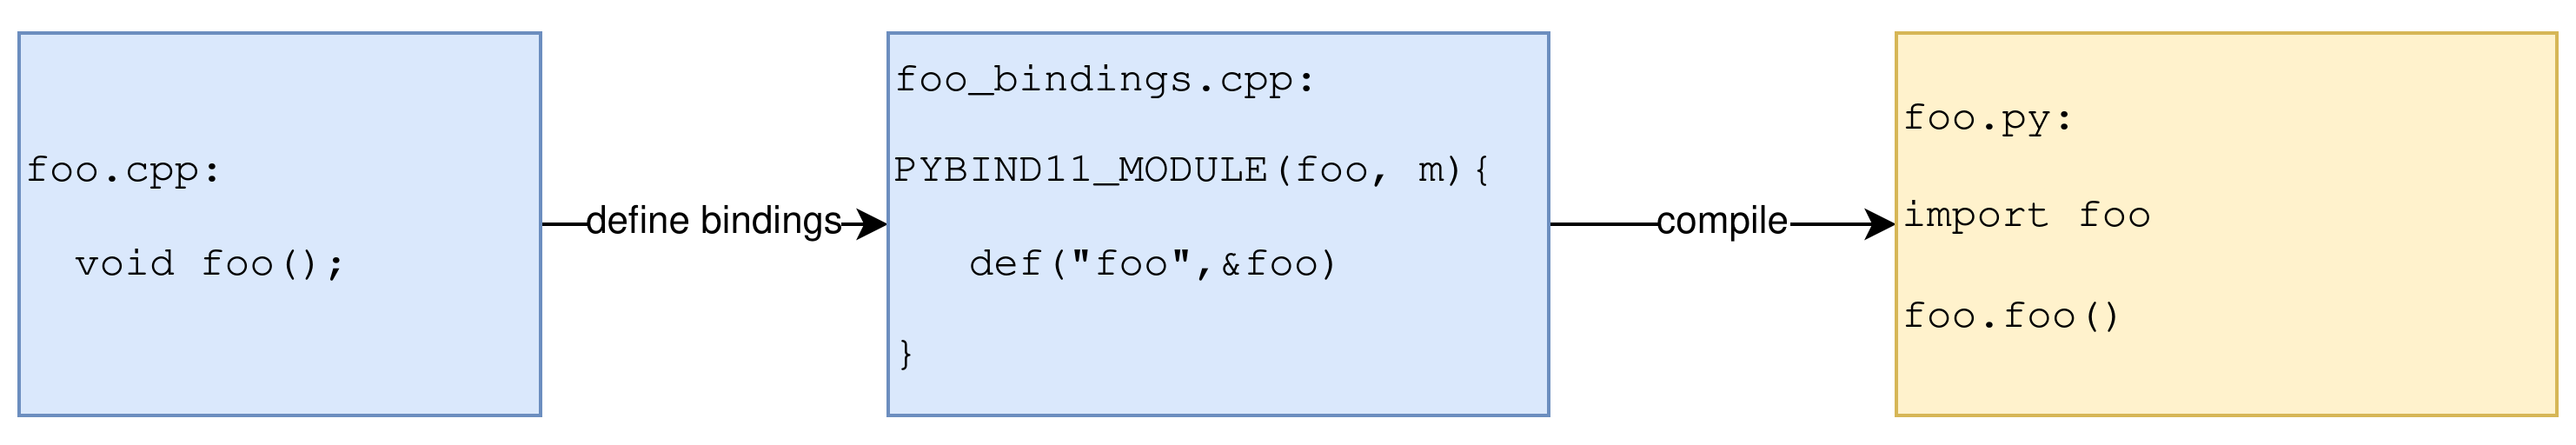
\includegraphics[width=\textwidth]{figures/pybind_schema.png}
    \caption{Pybind11 Schema}
    \label{fig:pybind11-schema}
\end{figure}



\subsubsection{Cython: Compiled Python Extensions}

Cython allows for the compilation of Python-like code into optimized C, potentially yielding performance improvements. It is suitable for creating C extensions and bridging Python with external C libraries. However, its effectiveness in wrapping existing C++ libraries may vary, as it may not fully leverage the library's pre-existing design.

\subsubsection{pybind11: Modern C++ Bindings}

pybind11 is a header-only library designed to simplify the creation of Python bindings for C++ code. It leverages compile-time introspection to minimize boilerplate and offers robust support for modern C++ features, including templates and \ac{STL} data structures. Its design prioritizes ease of use and maintainability.

\subsubsection{SWIG: Multi-Language Interface Generation}

SWIG is a tool capable of generating bindings for numerous programming languages. While it supports a broad range of C++ features, it introduces its own interface definition language, which may present a learning curve. Additionally, the necessity for manual type mappings can increase development effort.

\subsubsection{Py-C-API: Native Python Extensions}

The Python/C API provides a direct mechanism for extending the Python interpreter with C or C++ modules. While offering high performance, it demands meticulous memory management and can result in less readable code. It is generally better suited for creating custom extensions than for wrapping existing libraries.

\subsubsection{Alternative Binding Tools}

Other tools, such as Boost.Python and Cffi, offer alternative approaches. Boost.Python, while powerful, introduces complex installation process. Cffi, primarily designed for C, may not fully support the complexities of modern C++ libraries, particularly those utilizing modern C++ features.
\subsection{Performance Comparison}

Performance is a critical consideration, especially for tasks involving searching and updating components in large topologies. The overhead associated with each technology, including function calls and type casting, must be evaluated.

Initial tests involving file I/O operations indicate that Py-C-API offers the best performance, followed by pybind11 and SWIG. Python and Cython exhibit significantly lower performance due to the interpreter overhead.

Further benchmarks comparing SWIG and pybind11 for hierarchical component searches show that SWIG is generally faster, except when using smart pointers. However, pybind11's ease of use and maintainability outweigh the slight performance advantage of SWIG.


\subsection{Technology Decision: pybind11 for Optimal Integration}

The selection of pybind11 as the primary technology for creating Python bindings for the sys\_sage library stems from a comprehensive evaluation of various options, balancing performance, maintainability, and ease of use. While performance benchmarks indicated that SWIG might offer a slight speed advantage in certain scenarios, particularly with standard data structures, the crucial consideration of developer experience and long-term maintainability tipped the scales in favor of pybind11.

A significant drawback of SWIG is its reliance on a unique interface definition language. This necessitates that developers learn a new syntax, distinct from both C++ and Python, which can impede development speed and increase the learning curve for new contributors. In contrast, pybind11, being a header-only library embedded within C++, offers a more intuitive and familiar development environment for C++ programmers. This direct integration with C++ simplifies the process of creating and maintaining bindings, making it easier for future developers to understand and extend the project.

This decision aligns with findings from independent benchmarks, such as those presented in the \autoref{chapter:Related Work}, which highlight pybind11's superior usability despite potential performance trade-offs. The ease of integration and the reduced cognitive load for developers translate to faster development cycles and improved maintainability—critical factors for the long-term success of the sys\_sage library's Python interface.

Furthermore, pybind11's robust support for C++ features, including \ac{STL} containers and inheritance, aligns perfectly with the sys\_sage library's complexity. Its ability to seamlessly handle these features simplifies the wrapping process and ensures that the Python interface accurately reflects the C++ library's functionality. This comprehensive feature support, combined with its ease of use, makes pybind11 the optimal choice for creating a maintainable and extensible Python interface for the sys\_sage library.